
\documentclass[a4paper,12pt]{article}

\usepackage{graphicx} % Required for inserting images
\usepackage{amsmath,amssymb,amsfonts}
\usepackage{subcaption}
% -----------------------
% Package Imports
% -----------------------

% Set page margins
\usepackage[a4paper, top=1in, bottom=0.8in, left=1.1in, right=0.8in]{geometry}

% Use Times New Roman font
\usepackage{times}

% Add page numbering
\pagestyle{plain}

% Enable graphics inclusion
\usepackage{graphicx}
\usepackage{float}
% Enable code listings
\usepackage{listings}
\usepackage{xcolor} % For customizing code colors
\setlength{\parindent}{0pt}




\begin{document}
	\section{Experiment No. 4}
	
	\section{Experiment Title }
	External characteristic curve of compound DC Generator.
	\section{Objective}
	
	The objectives of this lab are as follows:
	\begin{itemize}
		\item To investigate the external characteristics of a compound DC generator.
		\item To analyze the variation in terminal voltage with respect to load current.
		\item To compare the behavior of cumulative over-compound, cumulative under-compound, and differential compound DC generators under varying load conditions.
	\end{itemize}
	
	\section{Theory}
	A compound generator is a type of DC generator that combines the characteristics of both shunt and series generators. It has two sets of field windings: the shunt winding and the series winding. The shunt winding is connected in parallel with the armature, while the series winding is connected in series with the armature. This configuration allows the compound generator to provide better voltage regulation and load characteristics compared to separately shunt or series generators.\\
A shunt generator is unsuitable where constancy of terminal voltage is essential, because its terminal voltage decreases as the load on it increases. This decrease in V is particularly objectionable for lighting circuit where even slight change in the voltage makes an appreciable change in the candle power of the incandescent lamps. A shunt generator may be made to supply substantially constant voltage (or even a  rise in voltage as the load increases) by adding to it a few turns joined in series with either the armature or the load (Figure-1). \\ 
\begin{figure}[H]
	\centering
	\begin{subfigure}[t]{0.48\textwidth}
		\centering
		\includegraphics[width=0.8\linewidth]{../../Others/screenshot0011}
		\caption{Compound DC Generator}
	\end{subfigure}
	\hfill
	\begin{subfigure}[t]{0.48\textwidth}
		\centering
	\includegraphics[width=0.6\linewidth]{../../Others/screenshot0010}
	\caption{ Characteristic curve of Compound DC Generator}
	\end{subfigure}
	
	\caption{Long Shunt and Short Shunt }
\end{figure}


These turns are so connected as to aid to shunt turns when the generator supplies load. As the load current increases, the current through the series windings also increase thereby increasing the flux. Due to the increase in flux, induced e.m.f. is also increased. By adjusting the number of series turns (or series amp-turns), this increase in e.m.f. can be made to balance the combined voltage drop in the generator due to armature reaction and the armature drop. Hence, V remains practically constant which means that field current is also almost unchanged. 

	

	
	\subsection{Types of Compound Generators}
	Compound generators can be classified into the following categories:
	\begin{figure}[H]
		\centering
		\includegraphics[width=0.35\linewidth]{../../Others/screenshot0013}
		\caption{Characteristic curve of DC Generators}
		\label{fig:screenshot0013}
	\end{figure}
	
	\begin{enumerate}
	\item \textbf{Cumulative Compound Generator}
	In a cumulative compound generator, the magnetic fields produced by the shunt and series windings are in the same direction, adding up to provide a stronger net magnetic field. This configuration results in better voltage regulation under varying loads. It is widely used in applications requiring steady voltage output, such as power distribution systems and lighting circuits.
	
\item  \textbf{Differential Compound Generator}
	In a differential compound generator, the magnetic fields produced by the shunt and series windings oppose each other, weakening the net magnetic field. As a result, the terminal voltage decreases with an increase in load. This type of generator is less common and is mainly used in specific applications where a controlled voltage drop is desired, such as in arc welding.
	\end{enumerate}

	
	\subsection{Compounding Characteristics}
	Based on the behavior of the generator under load, compound generators can be further classified into the following types:
	\begin{enumerate}
		\item  \textbf{Over-Compound Generator:}
	In an over-compound generator, the series winding is stronger, causing the terminal voltage to rise above the no-load voltage as the load increases. This type is ideal for long-distance power transmission, where higher voltage at the load end is required to compensate for line losses.
	
	\item \textbf{ Under-Compound Generator:}
	In an under-compound generator, the series winding is weaker than the shunt winding. The terminal voltage drops as the load increases, making it suitable for applications where a slight decrease in voltage is acceptable.
	
\item  \textbf{Flat-Compound Generator:}
	In a flat-compound generator, the series winding is designed to balance out the voltage drop caused by the load current, keeping the terminal voltage constant. This type is commonly used in power distribution systems and situations where a stable voltage is required.
	\end{enumerate}

	
	\subsection{Connection Configurations: Long Shunt and Short Shunt}
	Based on the connection of the shunt and series windings relative to the armature, compound generators are classified as long shunt or short shunt generators:
	\begin{figure}[H]
		\centering
		\begin{subfigure}[t]{0.48\textwidth}
			\centering
				\includegraphics[width=1\linewidth]{../../Others/screenshot0011}
			\caption{Long Shunt Compound Generator}
		\end{subfigure}
		\hfill
		\begin{subfigure}[t]{0.48\textwidth}
			\centering
				\includegraphics[width=1\linewidth]{../../Others/screenshot0011}
			\caption{Short Shunt Compound Generator}
		\end{subfigure}
		
		\caption{Long Shunt and Short Shunt Compound Generator }
	\end{figure}

	
	\begin{enumerate}
	\item  \textbf{Long Shunt Compound Generator:}
	In a long shunt compound generator, the shunt winding is connected in parallel with both the armature and series winding. This configuration allows the shunt winding to receive the entire terminal voltage, providing consistent voltage regulation under varying load conditions.
	
	\item  \textbf{Short Shunt Compound Generator:}
	In a short shunt compound generator, the shunt winding is connected in parallel with only the armature, not the series winding. This configuration affects the voltage regulation slightly, making it suitable for applications where a minor variation in voltage is permissible.
	
	\end{enumerate}


	

\newpage
	
	
	
	
	\section{Required Apparatus}
	\begin{enumerate}
		\item Variable Resistor (Ratings: Resistance: 5000$\Omega$, Current: 0.31A),
		\item Variable Resistor (Ratings: Resistance: $2\times 200$$\Omega$, Current: 1.58A),
		\item Variable Resistor (Ratings: Resistance: $3\times50\Omega$, Current: 3.16A),
		\item Variable Resistor (Ratings: Resistance: $50\Omega$, Current: 3.16A),
		\item Three Phase Power Supply (Ratings: Voltage: 400V, Current: 10A),
		\item Three Phase Power Supply (Ratings: Voltage: 400V, Current: 10A),	
		\item DC Multimeter (Ratings: Voltage: 600V, Current: 20A) 
		\item Three Phase Asynchronous Motor (Ratings: Power: 500W, Voltage: 400V/230V, Current: 1.8A/1.3A, Speed: 1380 rpm),
		\item DC Generator (Ratings: Power: 300W, Voltage: 220V, Current: 1.4A)
		\item Tacho-Generator (Ratings: Current: 0.07A max, Speed: 5000 rpm max).
	\end{enumerate}
	\section{Circuit Diagrram}
	\begin{figure}[H]
		\centering
		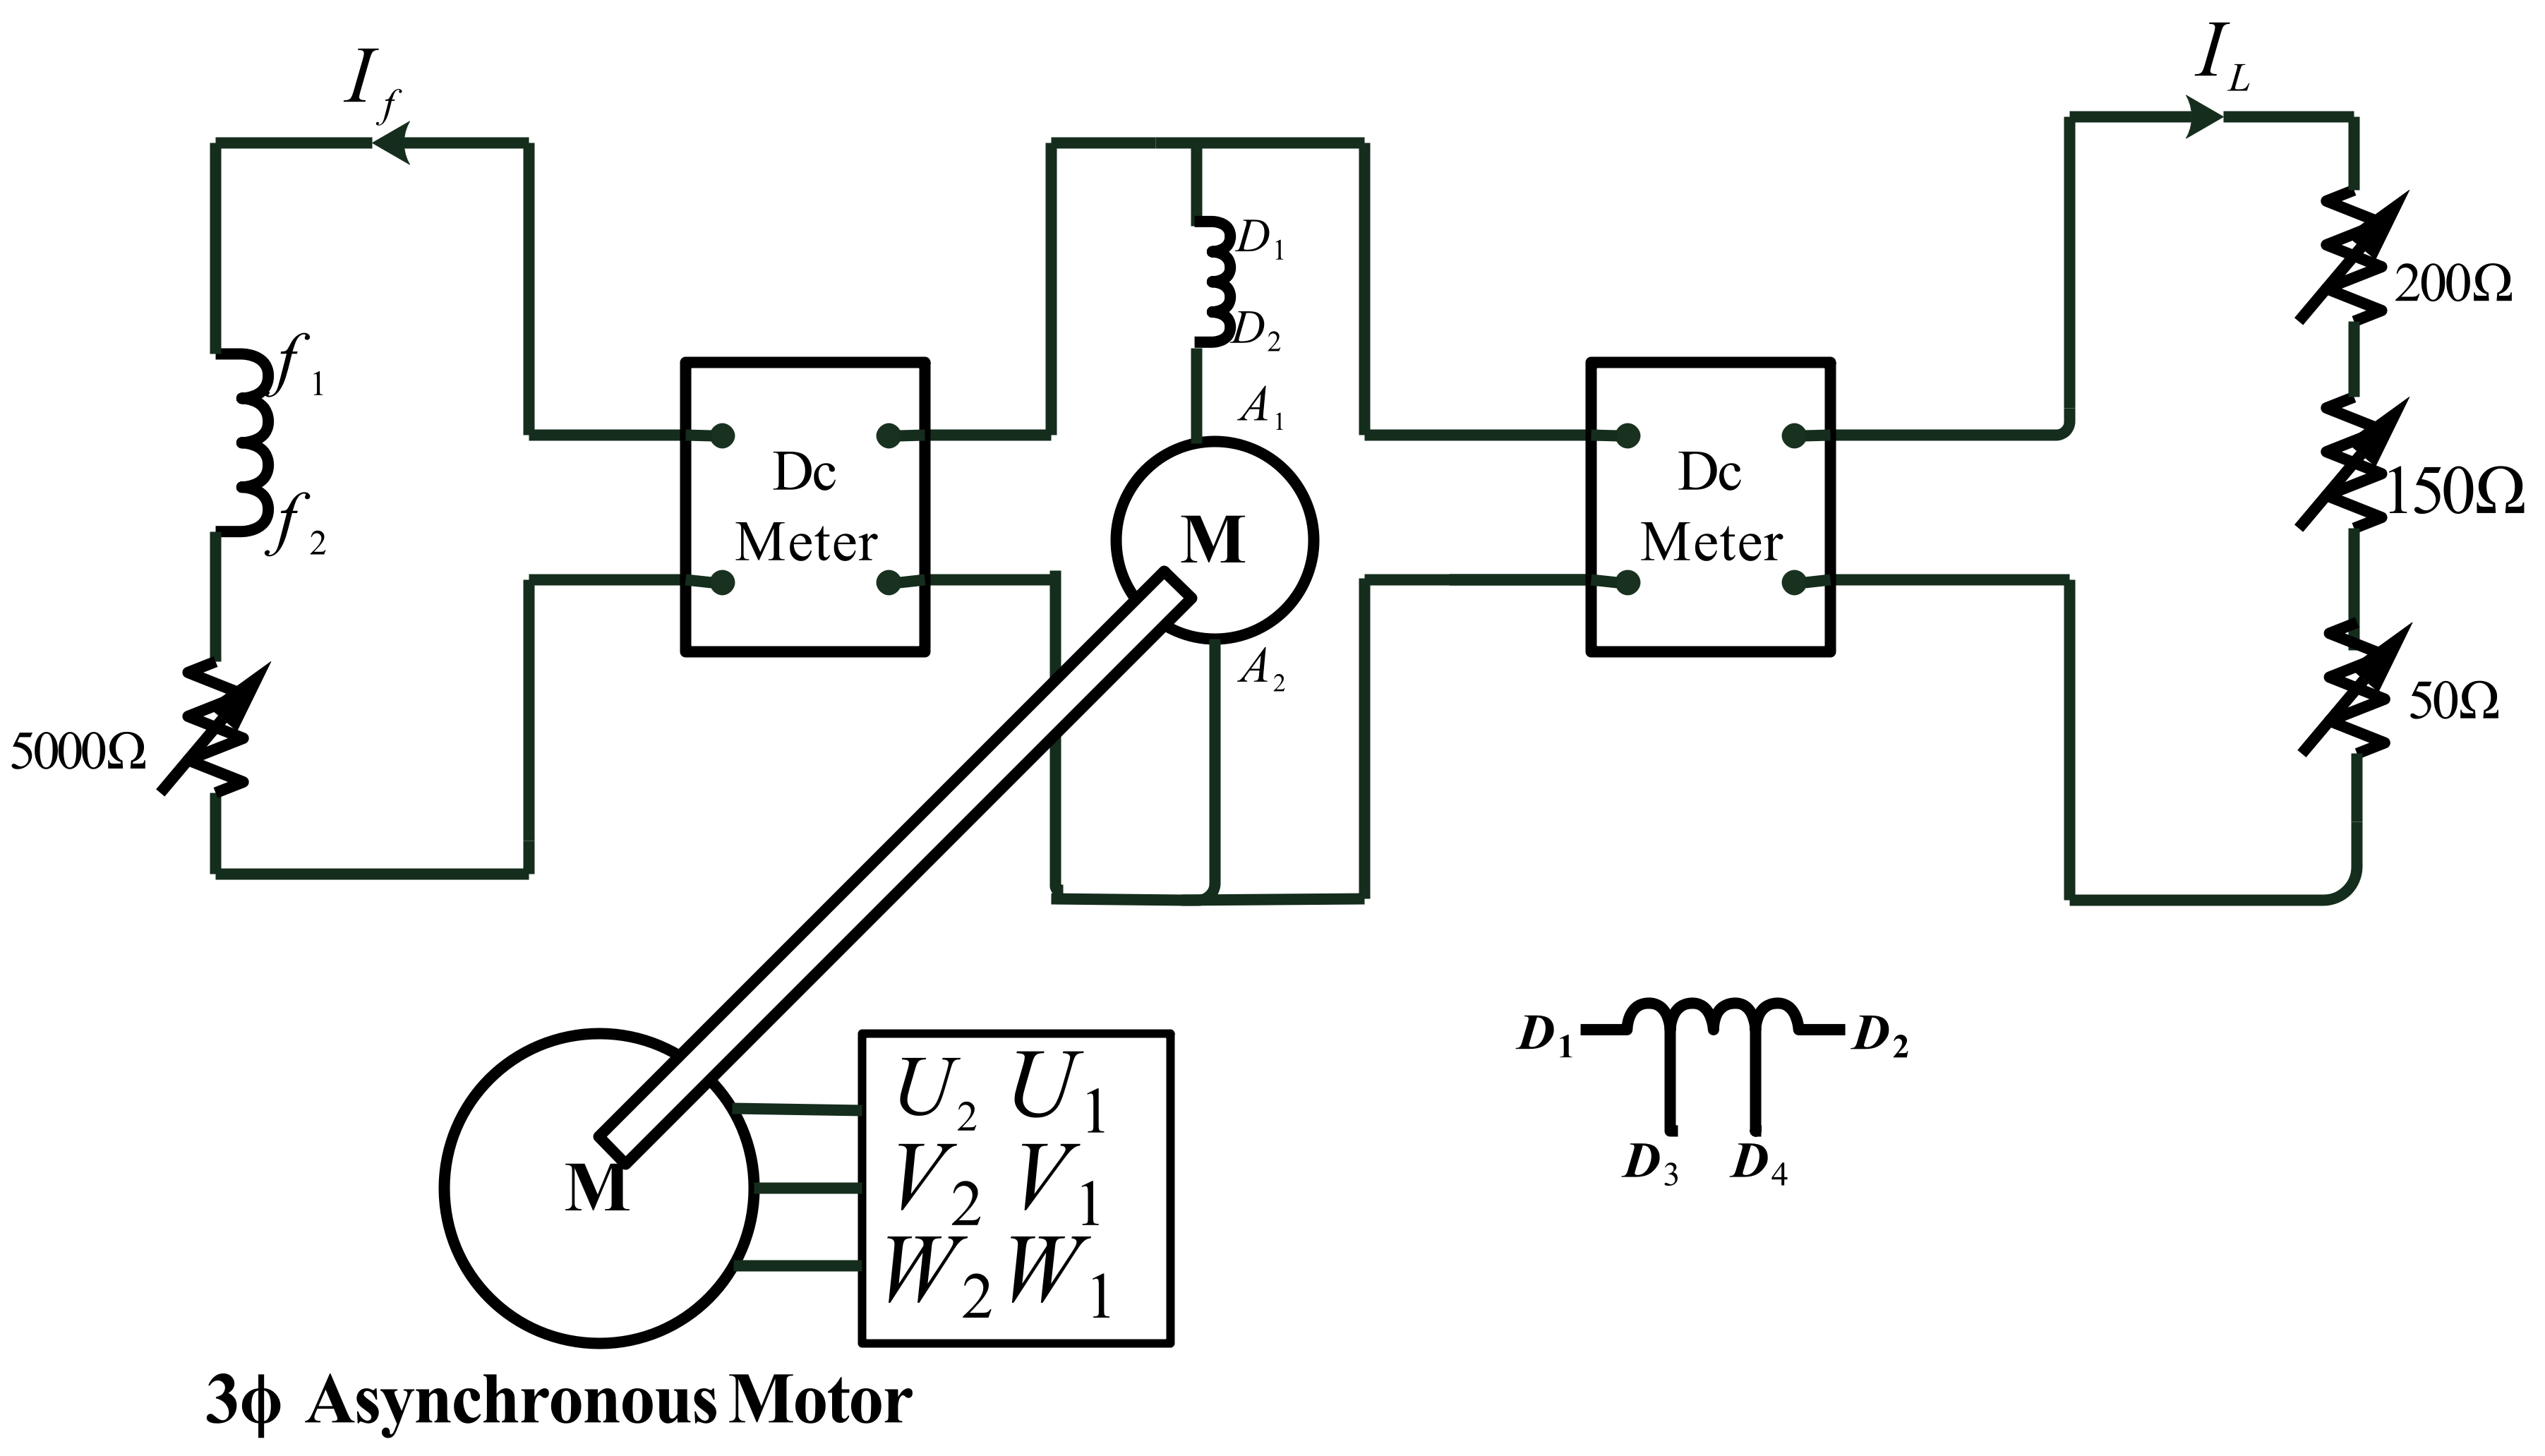
\includegraphics[width=1\linewidth]{Images/Drawing4}
	\caption{Required Circuit Diagram}
		
	\end{figure}
	
	

	
	
	\newpage
	\section{Data Table}
		\begin{table}[H]
		\centering
		\caption{Readings of  Terminal Voltage ($V_T$) and Load Current ($I_L$)}
		% Sub-table (a)
		\begin{subtable}[t]{0.45\textwidth} % Adjusted width for each sub-table
			\centering
			\begin{tabular}{|c|c|c|}
			\hline
			\multicolumn{1}{|c|}{\textbf{\begin{tabular}[c]{@{}c@{}}SL\\ No.\end{tabular}}} & \multicolumn{1}{c|}{\textbf{\begin{tabular}[c]{@{}c@{}}Terminal\\ Voltage\\ $V_T$\\(V)\end{tabular}}} & \multicolumn{1}{c|}{\textbf{\begin{tabular}[c]{@{}c@{}}Load\\ Current\\ $I_L$\\(A)\end{tabular}}} \\ \hline
			1                                                                               & 220.00                                                                                         & 0.00                                                                                      \\ \hline
			
			2                                                                               & 225.54                                                                                         & 0.542                                                                                      \\ \hline
			3                                                                              & 224.8                                                                                          & 0.575                                                                                      \\ \hline
			4                                                                               & 223.3                                                                                          & 0.655                                                                                      \\ \hline
			5                                                                               & 221.6                                                                                          & 0.740                                                                                      \\ \hline
			6                                                                               & 220.3                                                                                          & 0.794                                                                                      \\ \hline
			7                                                                               & 219.4                                                                                          & 0.847                                                                                      \\ \hline
			8                                                                               & 217.8                                                                                          & 0.907                                                                                      \\ \hline
			9                                                                               & 215.4                                                                                          & 1.03                                                                                       \\ \hline
			10                                                                               & 214.6                                                                                          & 1.06                                                                                       \\ \hline
			11                                                                              & 211.6                                                                                          & 1.20                                                                                       \\ \hline
			12                                                                              & 210.0                                                                                          & 1.247                                                                                      \\ \hline
			13                                                                              & 209.3                                                                                          & 1.279                                                                                      \\ \hline
			14                                                                              & 208.4                                                                                          & 1.30                                                                                        \\ \hline
			15                                                                              & 207.7                                                                                          & 1.33                                                                                       \\ \hline
			16                                                                              & 207                                                                                            & 1.34                                                                                       \\ \hline
		\end{tabular}
			\caption{Commulative [Under Compound] [$D_4-D_3$] } % Sub-table (a) caption
		\end{subtable}
		\hfil
		% Sub-table (b)
		\begin{subtable}[t]{0.32\textwidth} % Adjusted width for each sub-table
			\centering
			\begin{tabular}{|c|c|c|}
			\hline
			\multicolumn{1}{|c|}{\textbf{\begin{tabular}[c]{@{}c@{}}SL\\ No.\end{tabular}}} & \multicolumn{1}{c|}{\textbf{\begin{tabular}[c]{@{}c@{}}Terminal\\ Voltage\\ $V_T$\\(V)\end{tabular}}} & \multicolumn{1}{c|}{\textbf{\begin{tabular}[c]{@{}c@{}}Load\\ Current\\ $I_L$\\(A)\end{tabular}}} \\ \hline
			1           & 220.00         & 0.00        \\ \hline
			2           & 90.00       & 0.22        \\ \hline
			3           & 71.80       & 0.195       \\ \hline
			4           & 61.73       & 0.176       \\ \hline
			5           & 39.59       & 0.126       \\ \hline
			6           & 37.32       & 0.125       \\ \hline
			7           & 32.1        & 0.114       \\ \hline
			8           & 28.59       & 0.109       \\ \hline
			9           & 25.15       & 0.101       \\ \hline
			10          & 22.99       & 0.096       \\ \hline
			11          & 20.59       & 0.091       \\ \hline
			12          & 19.09       & 0.088       \\ \hline
			13          & 16.09       & 0.082       \\ \hline
			14          & 14.21       & 0.070       \\ \hline
			15          & 12.55       & 0.074       \\ \hline
		\end{tabular}
			\caption{Differential [$D_3-D_4$] } % Sub-table (b) caption
		\end{subtable}
		\hfil
		\begin{subtable}[t]{0.45\textwidth} % Adjusted width for each sub-table
			\centering
			\begin{tabular}{|c|c|c|}
			\hline
			\multicolumn{1}{|c|}{\textbf{\begin{tabular}[c]{@{}c@{}}SL\\ No.\end{tabular}}} & \multicolumn{1}{c|}{\textbf{\begin{tabular}[c]{@{}c@{}}Terminal\\ Voltage\\ $V_T$\\(V)\end{tabular}}} & \multicolumn{1}{c|}{\textbf{\begin{tabular}[c]{@{}c@{}}Load\\ Current\\ $I_L$\\(A)\end{tabular}}} \\ \hline
			
			
			1                                                         & 220.0       & 0.00       \\ \hline
			2                                                         & 254.3       & 0.629       \\ \hline
			3                                                         & 254.0       & 0.667       \\ \hline
			4                                                         & 253.3       & 0.727       \\ \hline
			5                                                         & 252.5       & 0.802       \\ \hline
			6                                                         & 251.5       & 0.876       \\ \hline
			7                                                         & 250.7       & 0.940       \\ \hline
			8                                                         & 250.0         & 1.00        \\ \hline
			9                                                         & 247.8       & 1.175       \\ \hline
			10                                                         & 247.6       & 1.22        \\ \hline
			11                                                        & 247.0       & 1.25        \\ \hline
			12                                                        & 246.4       & 1.283       \\ \hline
			13                                                        & 245.8       & 1.32        \\ \hline
			14                                                        & 245.6       & 1.33        \\ \hline
			15                                                        & 245.0         & 1.36        \\ \hline
		\end{tabular}
		\caption{Cmmulative [Over Compound] [$D_1-D_2$] }
		\end{subtable}
	\end{table}
	\section{Graph}
	
\begin{figure}[H]
	\centering
	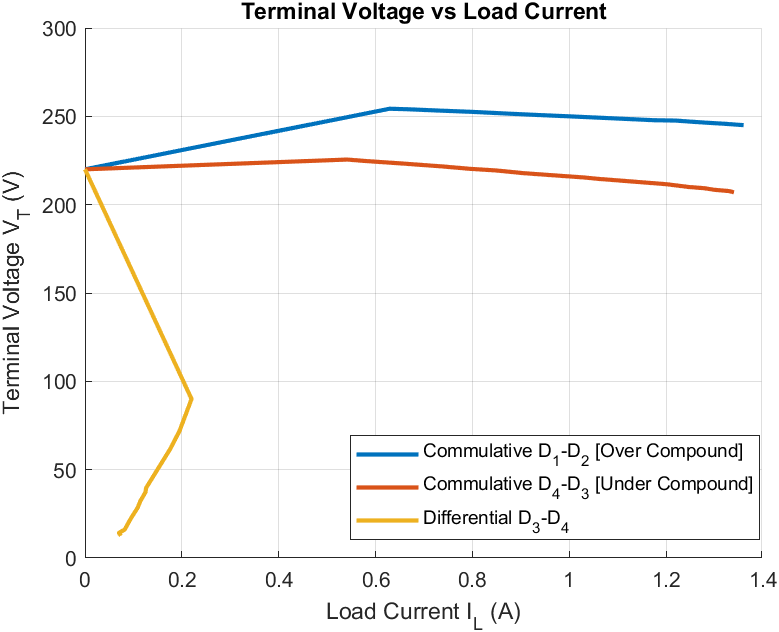
\includegraphics[width=0.9\linewidth]{Images/1}
	\caption{Terminal Voltage $(V_T)$ vs. Load Current $(I_L)$ characteristic curve}
	\label{fig:1}
\end{figure}
	\section{Discussion}
	The experiment was conducted to investigate the external characteristic curve of a compound DC generator. The relationship between the terminal voltage ($V_T$) and load current $(I_L)$ was analyzed. It was observed that as the load increased, the terminal voltage of the cumulative compound generator initially increased from 220V to 250.0V, before decreasing slightly to 245.0V. In the case of the cumulative under-compound generator, the terminal voltage ($V_T$) increased up to 225.54V and then fell to 207V as the load continued to increase. For the differential compound generator, the terminal voltage dropped abruptly from 220V to 90.0V and further decreased to 12.55V. The rated current of 1.4A was carefully monitored to ensure it did not exceed this value during the experiment as the load was incrementally increased. The results confirmed the distinct voltage regulation properties of each type of compound generator, influenced by factors such as residual magnetism, retentivity, and variations in speed.
\end{document}
